\section {Aufbau und Durchführung}
\label{sec:durchführung}

\subsection{Bestimmung der Schwingungsdauer ohne B-Feld}

Um die Schwingungsdauer zu bestimmen, wird die Messapparatur aus Abbildung \ref{fig:apparatur1} verwendet.

\begin{figure}
  \centering
  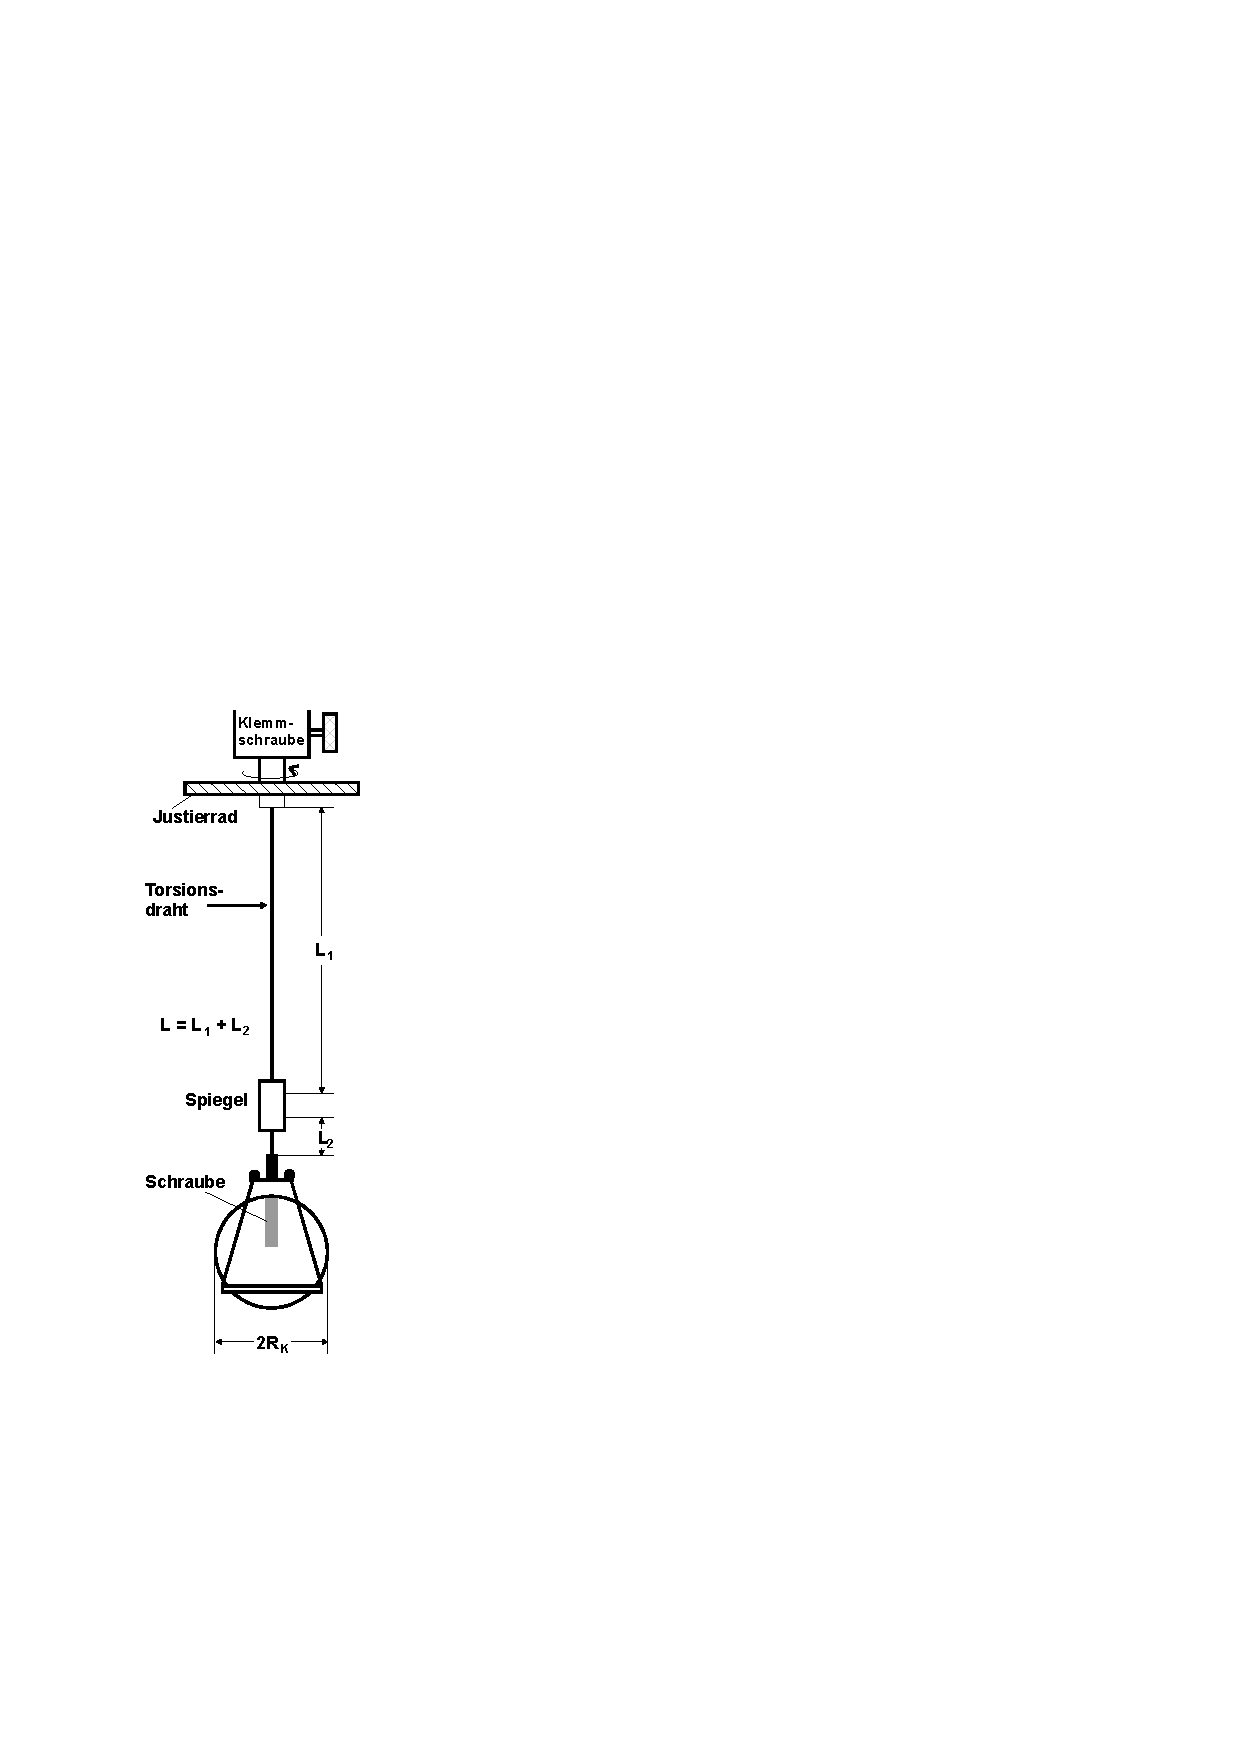
\includegraphics[scale=0.8]{bilder/messapparatur.pdf}
\caption{Messapparatur zur Bestimmung der Schwingungsdauer ohne Magnetfeld \cite{anleitung102}.}
  \label{fig:apparatur1}
\end{figure}

Das von der Lampe abgestrahlte Licht wird durch einen Spalt gebündelt und auf einen Spiegel geworfen, welcher das dieses auf einen Lichtdetektor reflektiert. Dieser sendet ein elektrisches Signal, sodass die Messung der Periodendauer beginnt. Trifft erneut ein Lichtstrahl auf den Lichtdetektor, wird die Zeit gestoppt. Abbildung \ref{fig:schematisch} zeigt den entsprechenden Aufbau.

\begin{figure}
  \centering
  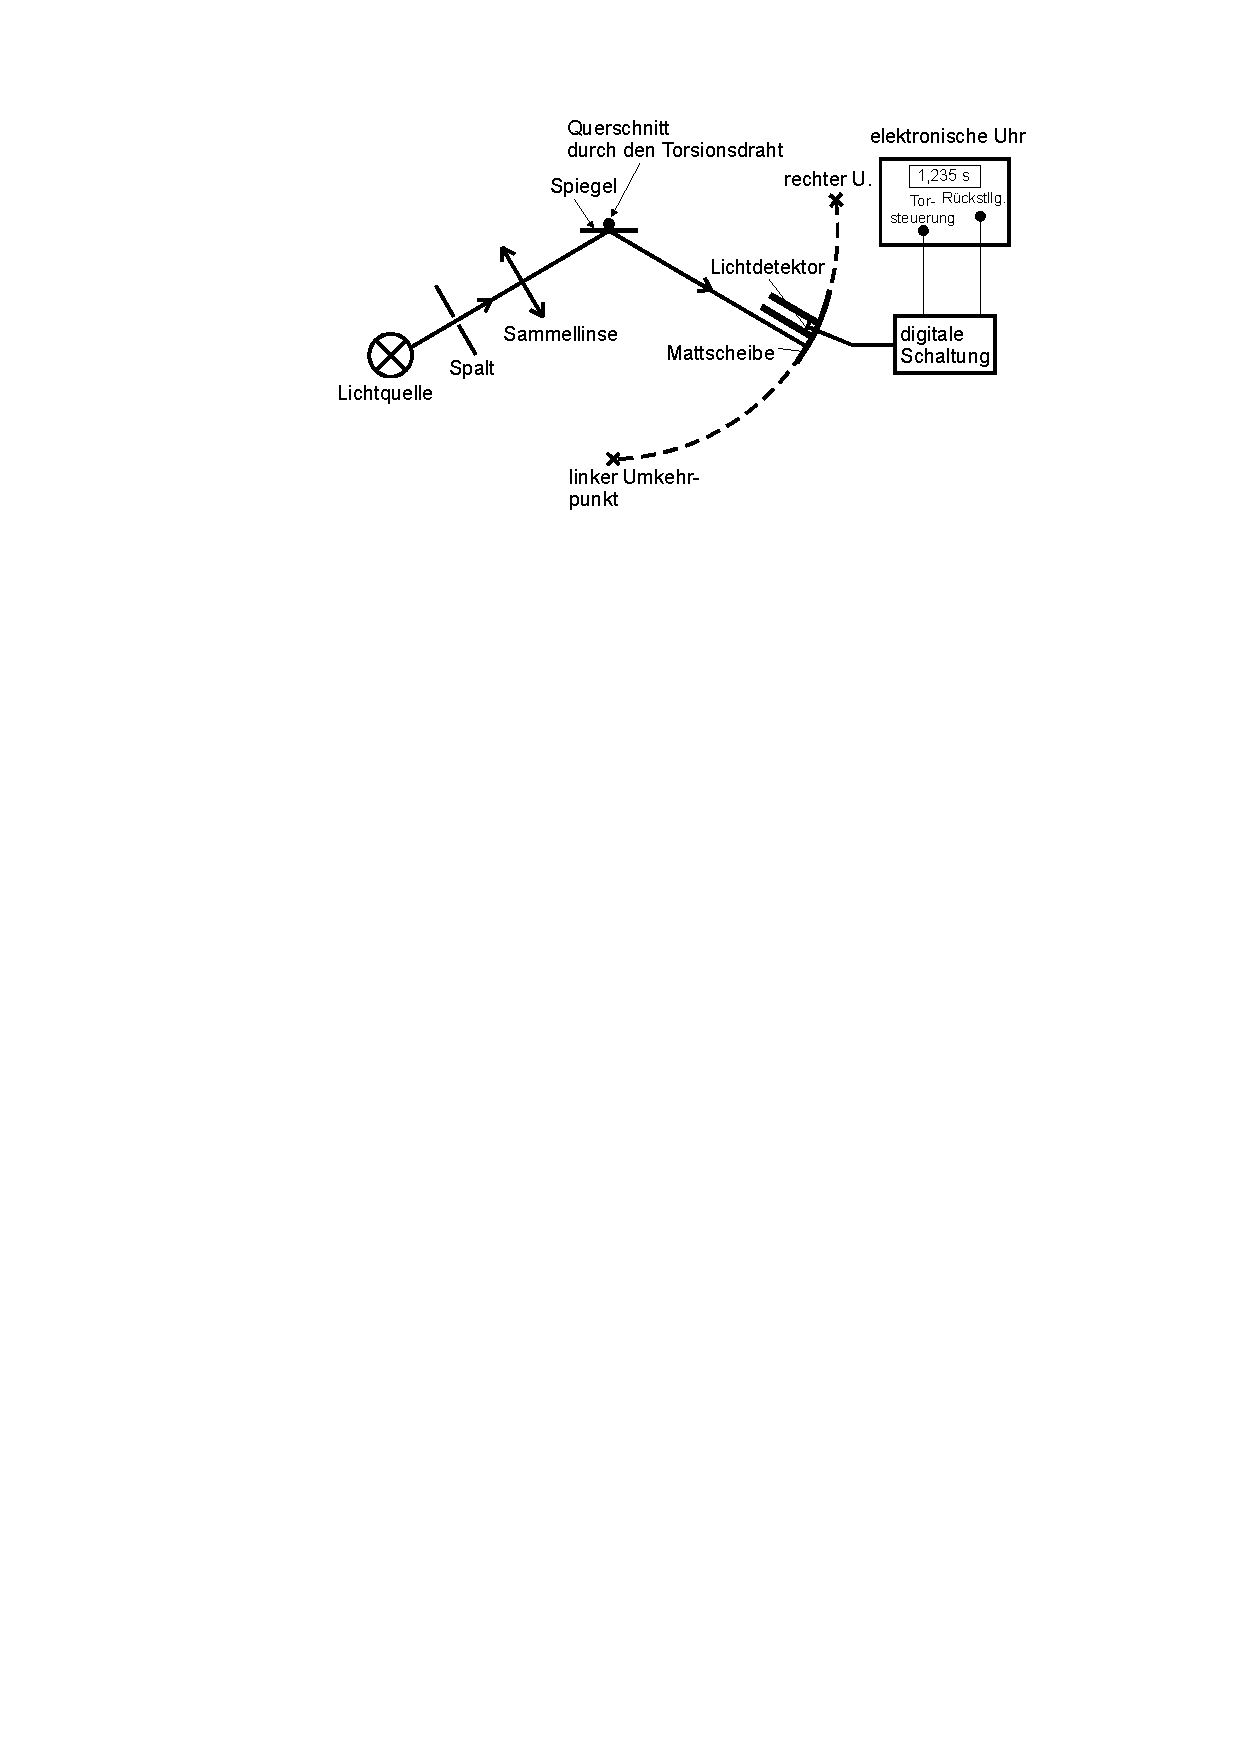
\includegraphics[scale=0.7]{bilder/messapparatur-schematisch.pdf}
\caption{Schematische Darstellung der Periodendauermessung \cite{anleitung102}.}
  \label{fig:schematisch}
\end{figure}

Da die Dauer einer Periode die Differenz der Zeit vom ersten und dritten elektrischen Signal ist, muss eine Schaltung entworfen werden, welche die Zeitmessung nicht bereits nach dem Zweiten beendet. Abbildung \ref{fig:TTL} zeigt die Schaltung aus TTL-Bausteinen, welche dies gewährleistet.

\begin{figure}
  \centering
  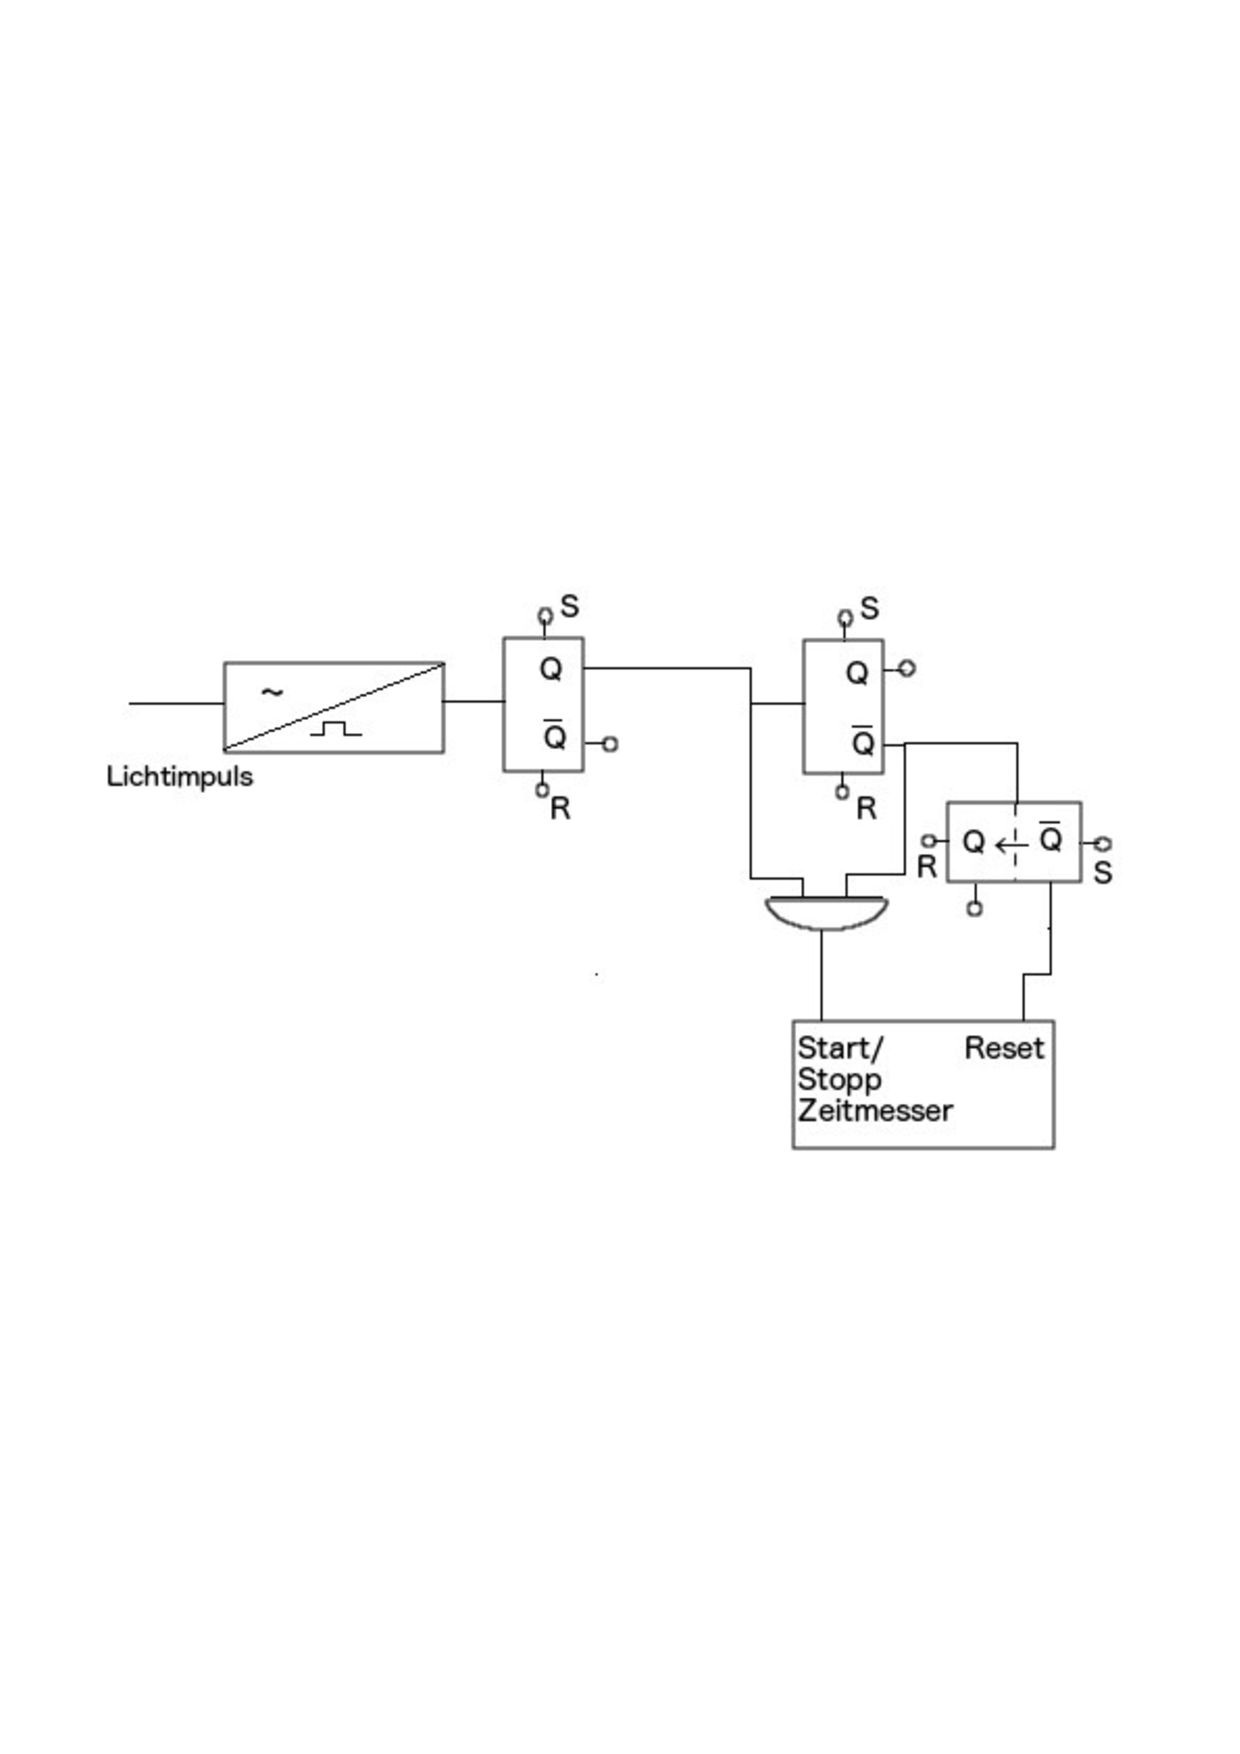
\includegraphics[scale=0.5]{bilder/schaltung-TTL.pdf}
\caption{Schaltung aus TTL-Bausteinen zur Steuerung der elektrischen Uhr \cite{anleitung102}.}
  \label{fig:TTL}
\end{figure}

Das zweite elektrische Signal wird durch eine bistabile Kippstufe unterdrückt. Somit wird beim dritten Signal die Zweitmessung gestoppt. Mithilfe einer weiteren bistabilen Kippstufe und einer monostabilen Kippstufe wird das vierte Signal für den Reset der Uhr genutzt.

Für die erste Messung zeigt die sich in der Kugel befindende Schraube in Richtung des Drahtes. Es ist zu beachten, dass die Kugel wegen der Kleinwinkelnäherung nur um kleine Winkel ausgelenkt werden darf. Mit Hilfe des Justierrades wird das System zum Schwingen angeregt. Mit Hilfe der vorher beschriebenen Schaltung wird die Periodendauer $T$ gemessen.

Die Messung wird mit Ausrichtung der Schraube senkrecht zum Draht in Nord-Süd Richtung wiederholt.

\subsection{Schwingungsdauer im regulierten Magnetfeld}

\begin{figure}
\centering
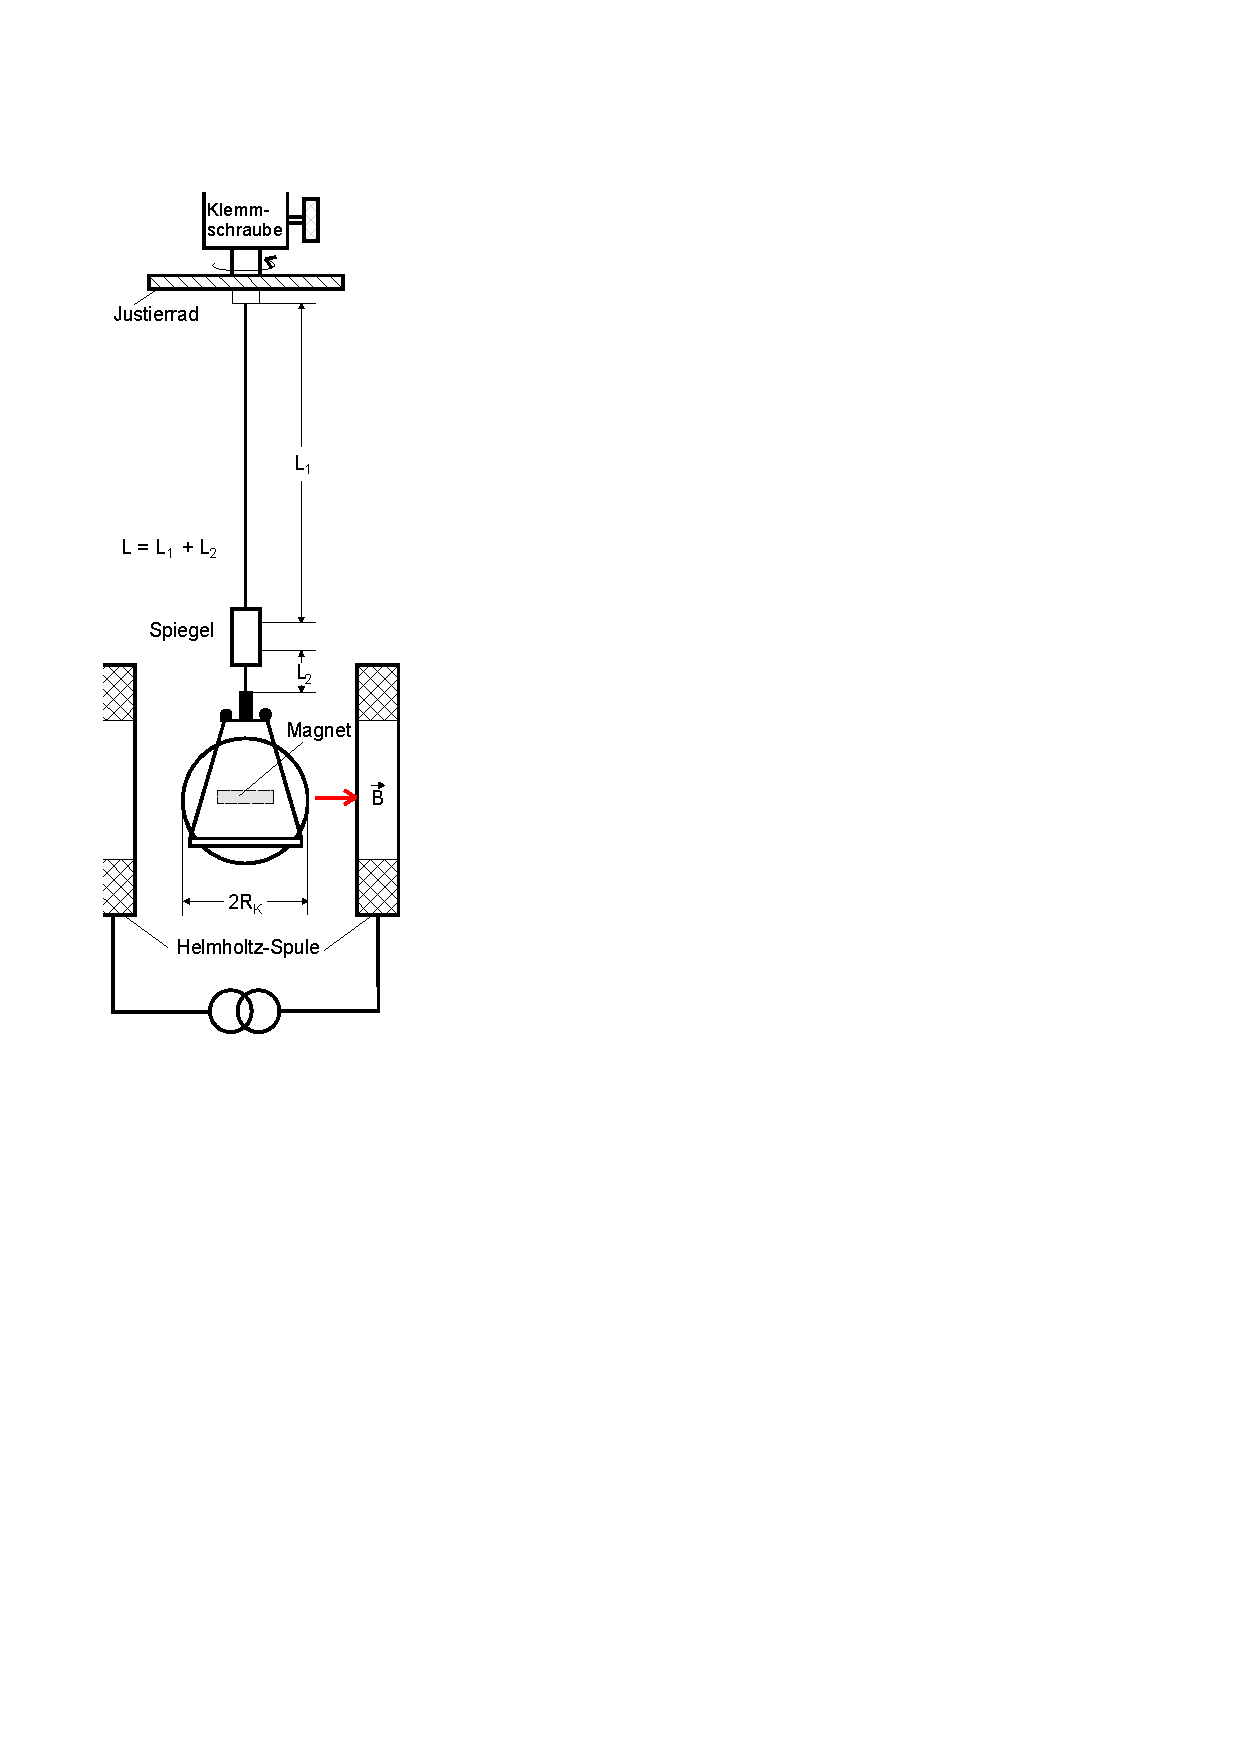
\includegraphics[scale=0.7]{bilder/apparatur2.pdf}
\caption{Messapparatur zur Bestimmung der Schwingungsdauer im regulierten Magnetfeld \cite{anleitung102}.}
  \label{fig:apparatur2}
\end{figure}

Der Aufbau zur vorherigen Messung unterscheidet sich lediglich durch eine eingebaute Helmholtz-Spule, welches ein homogenes Magnetfeld erzeugt. Die Schraube wird nun senkrecht zum Draht ausgerichtet, um Fehler durch den Einfluss des Erdmagnetfeldes zu verhindern. Im Bereich der Stromstärke von 0,5 - 5 \si{\ampere} werden fünf verschiedene Stromstärken eingestellt und jeweils acht Messwerte zur Schwingungsdauer aufgenommen.

\subsection{Bestimmung des Schubmoduls}
Um das Schubmodul bestimmen zu können, wird der Drahtdurchmesser mit einer Mikrometerschraube an drei verschiedenen Stellen gemessen.  Außerdem wird die Länge des Drahtes vom Justierrad bis zum Spiegel und vom Spiegel bis zur Halterung drei mal gemessen.
